\documentclass[../Article_Model_Parameters.tex]{subfiles}
\graphicspath{{\subfix{../Figures/}}}
\begin{document}

    {\color{blue}The solid-fluid extraction process is assumed to operate in a semi-continuous mode in a cylindrical vessel. In the extractor, essential oils are removed from biomass (for example, carqueja seeds) by supercritical carbon dioxide. As the solvent flows continuously through the bed of porous particles, the $CO_2$ molecules diffuse into the pores and adsorb on the particle surface to form an external fluid film around the solid particles. Then the solute dissolves and diffuses into the solvent in the pores and eventually into the bulk. The solvent-solute mixture leaves the extractor and undergoes depressurization. The $CO_2$ is released to a gaseous state, and the solute precipitates. In the vapour-liquid separator, the gaseous solvent is vent off while the precipitated product is collected.
		
		In Figure \ref{fig: SFE_drawing}, an instrumental set-up is presented. The flow rate ($F_{in}$) and the temperature ($T_{in}$) of the solvent entering the extractor are measured and can be adjusted using a pump and a heat exchanger, respectively. Moreover, the extractor's pressure ($P$) is assumed to be measurable and adjustable using a back-pressure regulator valve. In addition, the temperature of the outlet stream $T_{out}$ and the temperature profile of the fixed-bed can be measured. }
	
	\begin{figure}[h]
		\centering
		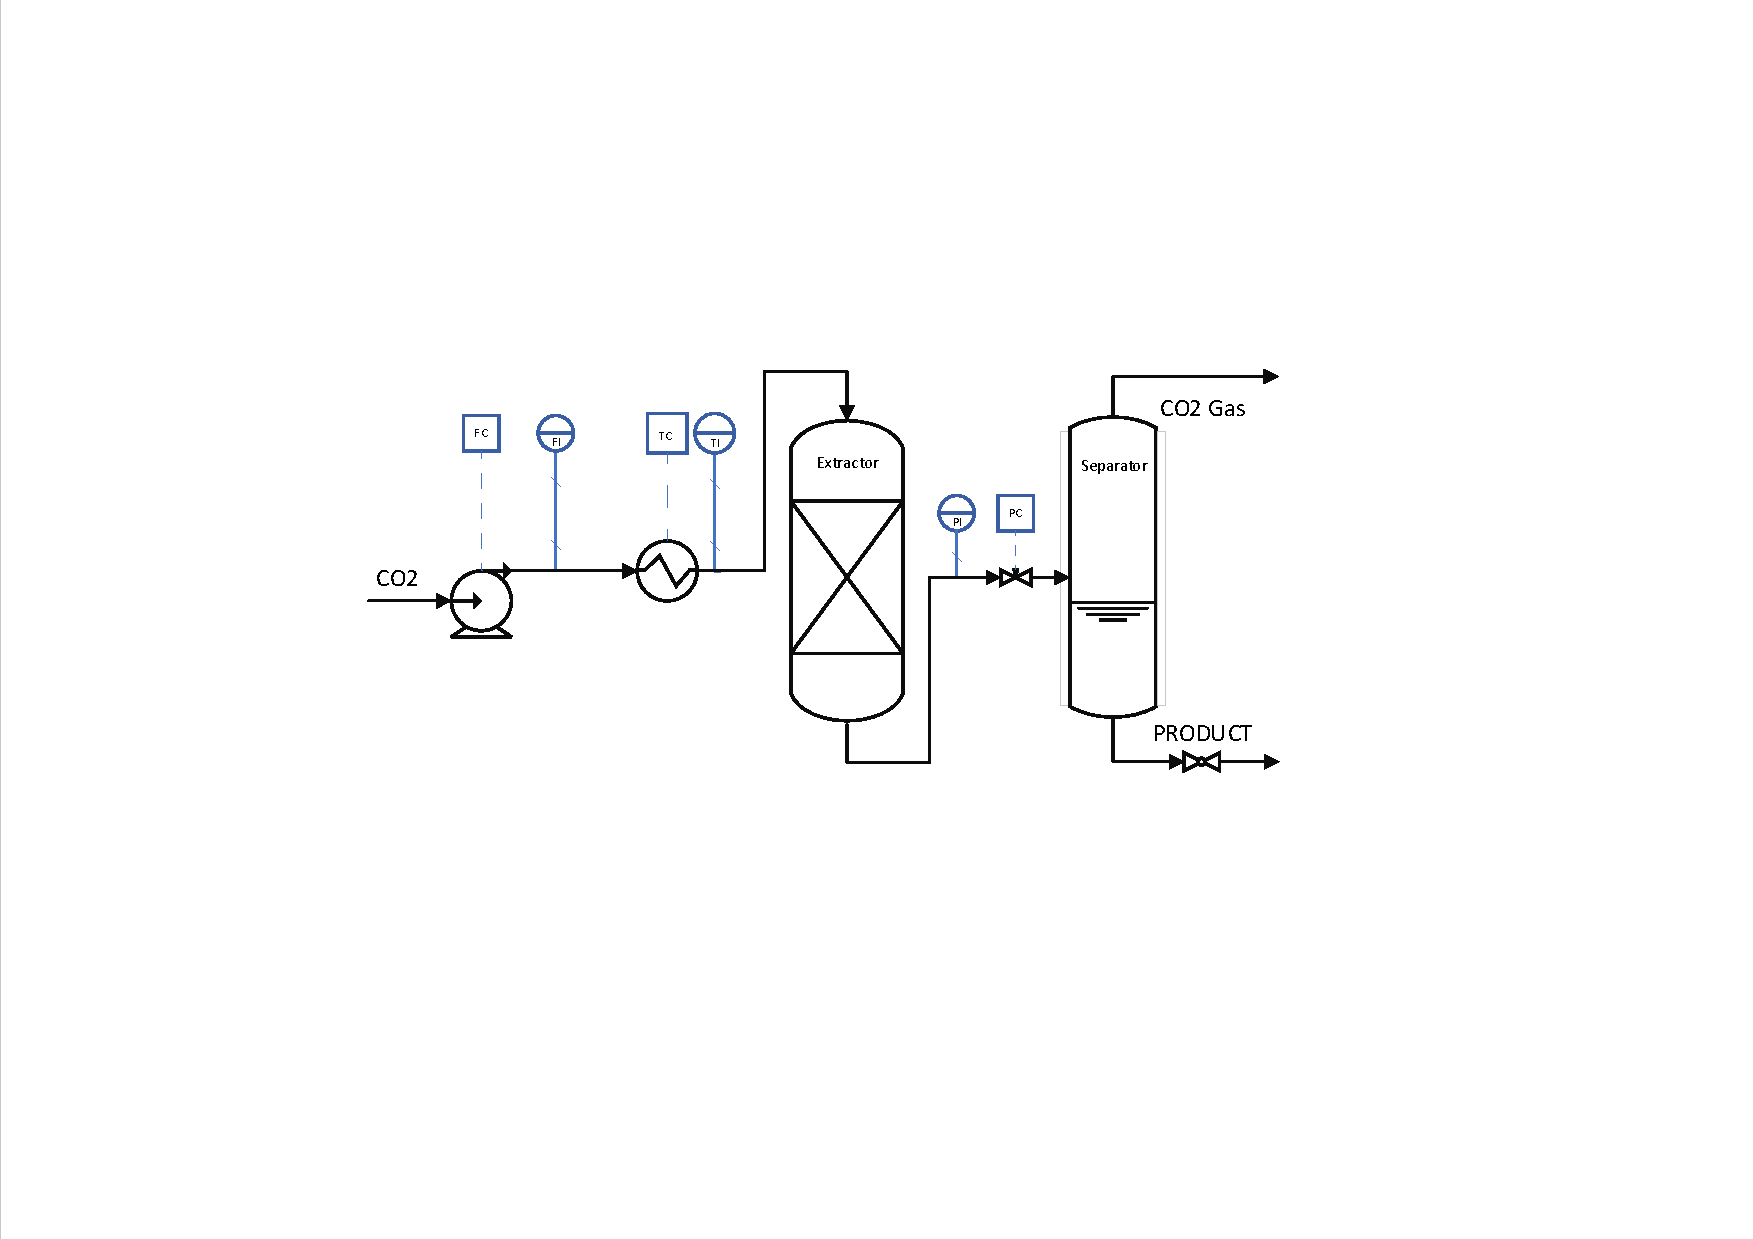
\includegraphics[trim = 6cm 7.5cm 8cm 6cm, clip, width=\linewidth]{SFE_PFD.pdf}
		\caption{Process flow diagram for solid-fluid extraction process}
		\label{fig: SFE_drawing}
	\end{figure}
	
	We consider a conventional solid-fluid extraction process in which soluble essential oils are removed from a solid matrix of biomass in super-critical carbon dioxide. A conventional configuration in which the extraction process is operated in semi-continuous mode typically may consist of an extraction vessel followed by a separation unit, like a fluid-solid flash drum. In the illustrative diagram in Fig. \ref{fig: SFE_drawing}, the solvent ($\text{CO}_2$ in super-critical conditions) is circulated through the, extractor in which it gets in contact with finely chopped biomass arranged on a fixed-bed. In the extractor, the solute (the essential oils) is firstly transferred from the solid phase to the fluid phase, then separated downstream in the drum and collected for further processing. The solvent from the drum can be recovered and recycled into the process. In Fig. \ref{fig: SFE_drawing}, we also depict a typical instrumentation set-up used to configure the operating conditions of the process and to monitor and control it: The flow-rate ($F_\text{in}$) and the temperature ($T_\text{in}$) of the solvent entering the extractor are expected to be measured and adjustable, for example using a pump and a heat exchanger as actuators, respectively. Moreover, it is expected that the pressure ($P$) in the extractor is measured and adjustable, for example using a back-pressure regulator valve. Basic process regulation can be achieved with PID controllers whose set-points are manually provided, whereas a more advanced control strategy would include a supervisory controller to optimally determine the set-points.
	\begin{figure}[h]
		\begin{center}
			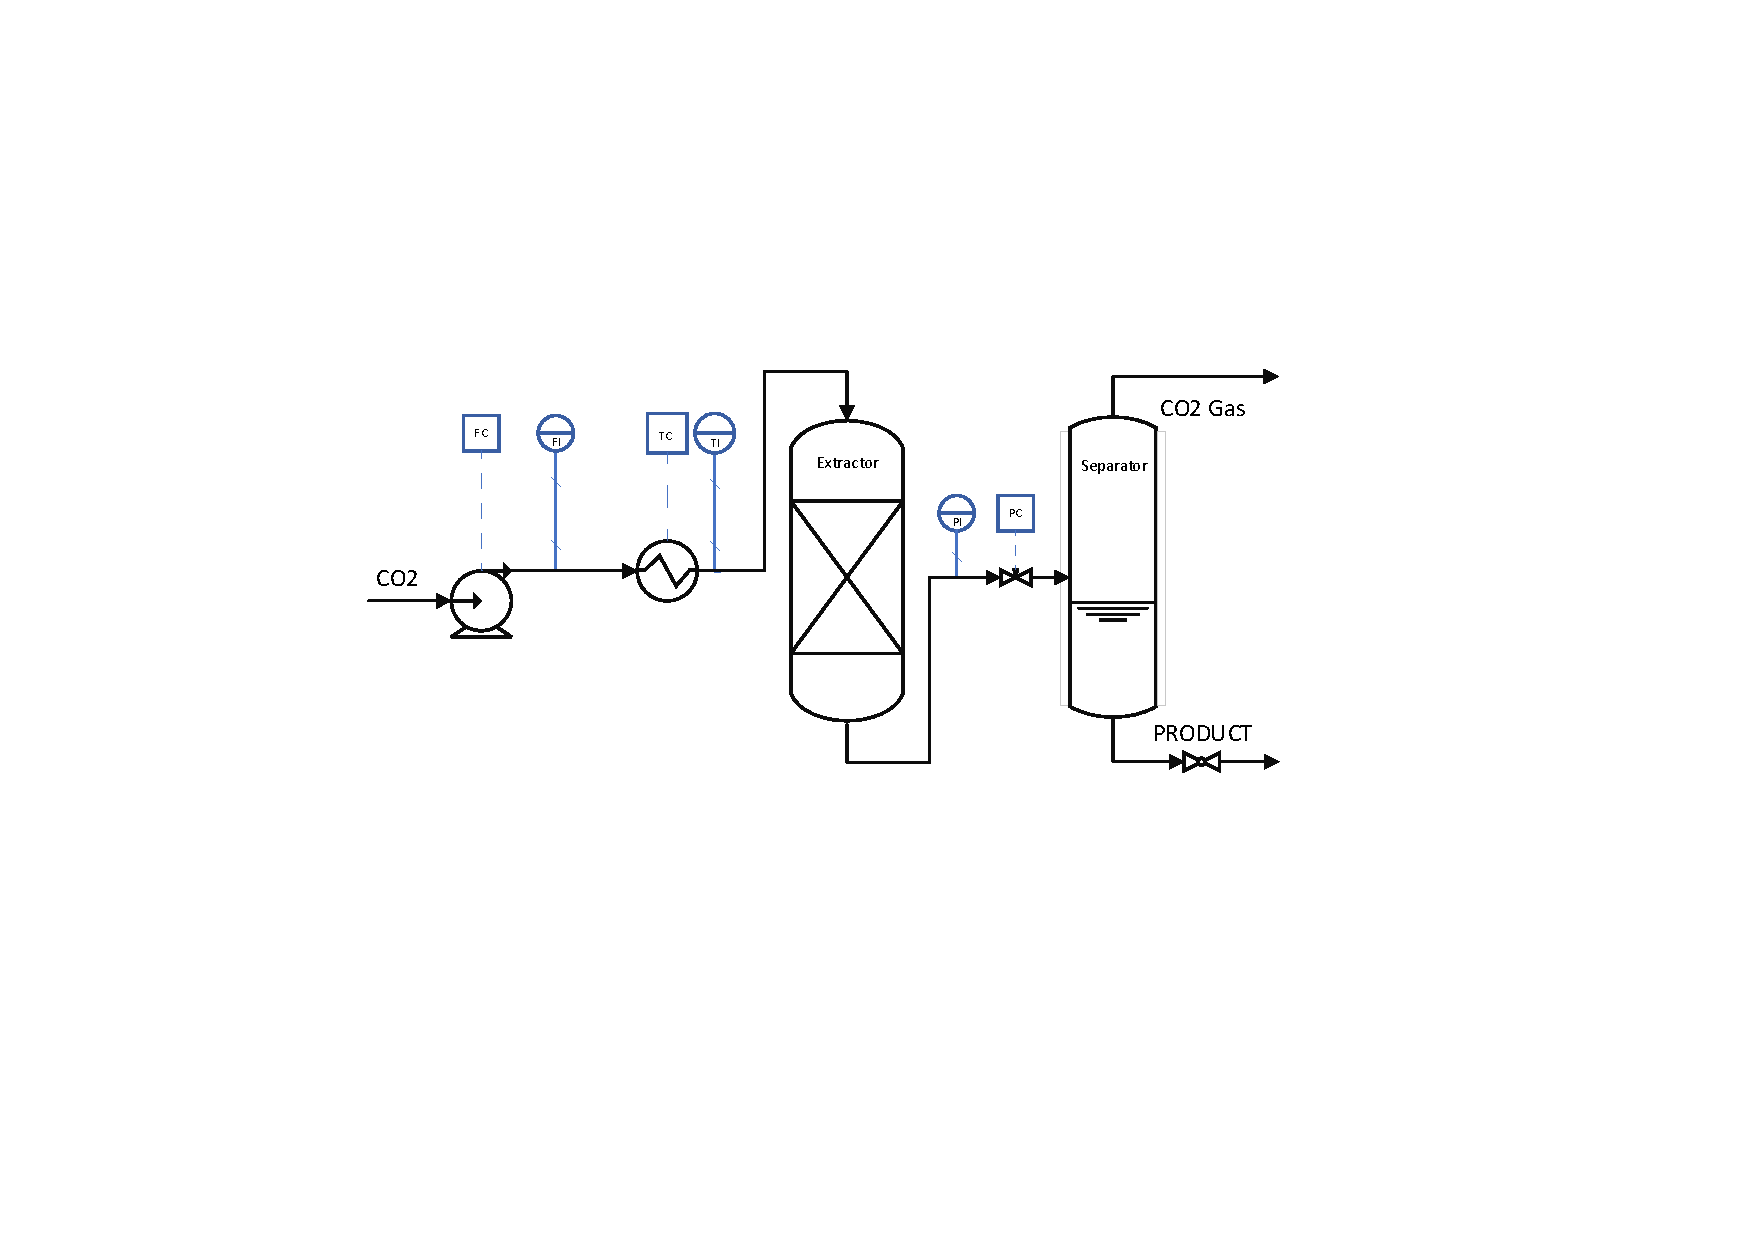
\includegraphics[width=0.66\linewidth]{Figures/SFE_PFD_cropped.pdf}
			\caption{Solid-fluid extraction process: Simplified process diagram and essential instrumentation.}
			\label{fig: SFE_drawing}
		\end{center}
	\end{figure}
	
	As solvent influent flow-rate and temperature, together with the pressure in the extractor, are understood as the main conditions that characterise the process from an operational point of view, we are interested in how these quantities affect the extraction process. More specifically, we are interested in understanding how they can be used in a supervisory control strategy based on a dynamic model of the extractor. The study is based on a forward sensitivity analysis (Section \ref{sec: State-space and sensitivity}) of a pragmatically designed model of the system. In Subsection \ref{subsec: Extraction model} and \ref{subsec: Measurement model}, the distributed-parameter model and the measurement model used for the task are presented. 
	
	\subsection{Extraction model} \label{subsec: Extraction model}
	We consider an operational description of the fluid-solid extraction process in the extractor developed from a distributed-parameter model with three partial differential equations: Namely, two mass balance equations, relative to concentration of solute in the fixed solid phase and in the mobile fluid phase, and the heat balance equation, relative to the temperature of the fluid phase. We assume that the fluid, a mixture of solute and solvent, in the extractor can be treated as a pseudo-homogenous phase whose properties are those of the dominant component, the solvent. A single pseudo-component collectively representing the extract is also used. \\
	
	For the convection of the fluid phase, we consider a plug-flow model of the velocity profile. Furthermore, we assume that no pressure drops and no heat losses occur along the extractor. We also limit the model to represent only axial diffusion for both mass and heat. As for the mass transfer from the solid to the fluid phase, an extraction term based on the two-film theory is used.  Being the solid phase fixed, the convection and diffusion terms in the corresponding mass balance are both exlcuded. Similarly, we assume that the extraction is an isothermal process and exclude the generative term from the heat balance. The particle size distribution, and thus the void fraction of the solid phase, is assumed to be uniform in space and to remain constant in time. \\
	
	Under these fairly general and simplifying assumptions, a macroscopic model of the extractor's bed reads
	
	\begin{subequations}\begin{align}
			\cfrac{\partial {\color{blue}c_{\text{F}}}(t,z)}{\partial t} &	= -\cfrac{1}{{\color{magenta}\varepsilon A}}\cfrac{{\color{red}F}(t)}{{\color{orange}\rho_\text{F}}\left[{\color{blue}T}(t,z),{\color{red}P}(t)\right]} \cfrac{\partial {\color{blue}c_{\text{F}}}(t,z)}{\partial{\color{blue}z}}
			+ {\color{orange}D^M_{\text{eff}}}\left[{\color{blue}T}(t,z),{\color{red}P}(t),{\color{red}F}(t)\right] \cfrac{\partial^2 {\color{blue}c_{\text{F}}}(t,z)}{\partial {\color{blue}z^2}}
			+ \cfrac{1-{\color{magenta}\varepsilon}}{{\color{magenta}\varepsilon}}{\color{blue}r_e}(t,z)	\label{eq: Model fluid} \\
			\cfrac{\partial {\color{blue}c_{\text{S}}}(t,z)}{\partial t} &	= {\color{blue}r_e}(t,z)		\label{eq: Model solid} \\
			\cfrac{\partial {\color{blue}T}(t,z)}{\partial t} &	= -\cfrac{{\color{red}F}(t) {\color{orange}C_p^\text{F}}\left[{\color{blue}T}(t,z),{\color{red}P}(t)\right]}{{\color{magenta}A} [(1-{\color{magenta}\varepsilon}){\color{orange}\rho_\text{F}}\left[{\color{blue}T}(t,z),{\color{red}P}(t)\right] {\color{orange}C_p^\text{F}} \left[{\color{blue}T}(t,z),{\color{red}P}(t)\right] + {\color{magenta}\varepsilon}{\color{magenta}\rho_\text{S}}{\color{magenta}C_p^\text{S} } ]} \cfrac{\partial {\color{blue}T}(t,z)}{\partial {\color{blue}z}} 
			+ {\color{orange}D^T_{\text{eff}}}\left[{\color{blue}T}(t,z),{\color{red}P}(t)\right] \cfrac{\partial^2 {\color{blue}T}(t,z)}{\partial {\color{blue}z^2}}	\label{eq: Model heat}
		\end{align}\label{eq: SFE model}\end{subequations}
	
	where ${\color{blue}c_{\text{F}}}(t,z)$, ${\color{blue}c_{\text{S}}}(t,z)$, and ${\color{blue}T}(t,z)$ denote respectively the concentration of solute in the fluid, concentration of solute in the solid, and temperature of the pseudo-homogeneous phase, all at axial positions $z \in [0,L]$ along the bed and at times $t \in [t_{\text{ini}},t_{\text{end}}]$. We use ${\color{magenta}A}$ to denote the cross-section of the bed, $L$ will be used to denote its length. The void fraction of the bed is denoted by ${\color{magenta}\varepsilon}$, whereas ${\color{magenta}\rho_\text{S}}$  and ${\color{magenta}C_p^\text{S} }$ are used to denote the density and the specific heat of the solid phase: These quantities are assumed to be known and to remain constant in space and time. We collectively denote these quantities as $\varphi_{\text{exp}} = \left(A,L,\varepsilon,\rho_{\text{S}},C^{\text{S}}_p\right)$.  ${\color{red}F}(t) = F_\text{in}(t)$ denotes the mass flow-rate through the extractor and ${\color{red}P}(t)$ its pressure: Together with the feed temperature $T(t,z=0) = T_{\text{in}}(t)$, these three variables define the process operating conditions and can be varied over time to control the extraction. \\
	
	The density ${\color{orange}\rho_\text{F}}\left[{\color{blue}T}(t,z),{\color{red}P}(t)\right]$ of the fluid phase, the axial mass diffusion coefficient $ {\color{orange}D^M_{\text{eff}}}\left[{\color{blue}T}(t,z),{\color{red}P}(t),\right]$, the specific heat ${\color{orange}C_p^\text{F}}\left[T(t,z),P(t)\right]$ of the fluid phase, and the axial heat diffusion coefficient ${\color{orange}D_{\text{eff}}^T}\left[T(t,z),P(t)\right]$ are assumed to change in space and over time, due to their dependence on the local temperature $T(t,z)$, and on pressure $P(t)$ and mass flow-rate $F(t)$. Similarly, the term ${\color{blue}r_e}(t,z)$ used to model the rate of extraction is assumed to vary in space and time, due to its dependence on the concentrations ${\color{blue}c_{\text{F}}}(t,z)$ and ${\color{blue}c_{\text{S}}}(t,z)$ of solute. \\
	
	The differential model in Eq. \eqref{eq: SFE model} augments what commonly found in the literature ({\color{red}ADD REFS}) in relation to mass balances (Eq. \eqref{eq: Model fluid} and \eqref{eq: Model solid}), by adding a heat balance (Eq. \eqref{eq: Model heat}) to describe changes in the concentrations of solute and temperature due to a potentially varying temperature of the influent solvent and pressure in the extractor. Because of the generality of the formulation, conventional relationships commonly found in the literature can used to describe the extraction rate, density and heat capacity in the fluid phase, and the diffusion coefficients: The specific choices used in this study are overviewed in the following subsections. To describe the properties of the fluid phase and to account for the aforementioned dependencies, an equation of state must be selected: In Subsection \ref{subsubsec: Equation of state}, we overview how we used the Peng-Robinson's equation for this task. As for the extraction rate, we overview in Subsection \ref{subsubsec: Extraction rate}
	
	\subsubsection{Equation of state and properties of the fluid phase} \label{subsubsec: Equation of state}
	We consider equations of state in the general form ${\color{red}P}(t) {\color{orange}V_{\text{CO}_2}}\left[T(t,z),P(t)\right] = {\color{orange}Z}{\color{magenta}R}{\color{blue}T}(t,z)$, where ${\color{magenta}V_{\text{CO}_2}}$ denotes the molar volume of $\text{CO}_2$, ${\color{orange}Z}$ represents its compressibility factor, and $R$ is the universal gas constant. More specifically, we are interested in these equations because of the possibility to express the compressibility $Z$ as an explicit function of temperature and pressure. This is the case when $Z$ is obtained as one of the physically meaningful roots of a polynomial equation, like the Peng-Robinson's and {\color{red} stuff with REFS to equations of state}. \\
	
	In Peng-Robinson's equation, the compressibility ${\color{orange}\overline{Z}}\left[{\color{blue}T}(t,z), {\color{red}P}(t)\right]$ solves the third-order polynomial equation
	\vskip-0.500cm
	
	\begin{equation}\label{eq: Compressibility}
		{\color{orange}Z}^3 - \left[1 - {\color{orange}B}\left[{\color{blue}T}(t,z), {\color{red}P}(t)\right]\right] {\color{orange}Z}^2 + \left[{\color{orange}A}\left[{\color{blue}T}(t,z), {\color{red}P}(t)\right] - 2{\color{orange}B}\left[{\color{blue}T}(t,z), {\color{red}P}(t)\right] - 3{\color{orange}B}\left[{\color{blue}T}(t,z), {\color{red}P}(t)\right]^2\right] {\color{orange}Z} = 0, 
	\end{equation}

	where ${\color{orange}A}\left[{\color{blue}T}(t,z), {\color{red}P}(t)\right]$ and ${\color{orange}B}\left[{\color{blue}T}(t,z), {\color{red}P}(t)\right]$ are functions of time and space defined on the attraction parameter, ${\color{orange}a}\left[{\color{blue}T}(t,z)\right] = {\color{magenta}a^c_{\text{CO}_2}}{\color{orange}\alpha}\left[{\color{blue}T}(t,z)\right]$ with ${\color{magenta}a^c_{\text{CO}_2}} \approx 0.45724 {{\color{magenta}R}^2{\color{magenta}T^c_{\text{CO}_2}}^2}/{{\color{magenta}P^c_{\text{CO}_2}}}$, and the repulsion parameter, ${\color{magenta}b_{\text{CO}_2}} \approx 0.07780 {{\color{magenta}R}{\color{magenta}T^c_{\text{CO}_2}}}/{{\color{magenta}P^c_{\text{CO}_2}}}$, both functions of the critical temperature ${\color{magenta}T^c_{\text{CO}_2}}$ and pressure ${\color{magenta}P^c_{\text{CO}_2}}$. Specifically, we have
	\vskip-0.250cm
	\begin{subequations} \label{eq: PR_AB}
		\begin{align} 
			{\color{orange}A}\left[{\color{blue}T}(t,z), {\color{red}P}(t)\right]	& = \dfrac{{\color{orange}\alpha}\left[T\left(t,z\right)\right]{\color{magenta}a^c_{\text{CO}_2}}{\color{red}P}(t)}{{\color{magenta}R}^2{\color{blue}T}^2(t,z)};													\label{eq: PR_A}\\
			{\color{orange}B}\left[{\color{blue}T}(t,z), {\color{red}P}(t)\right]	& = \dfrac{{\color{magenta}b_{\text{CO}_2}}{\color{red}P}(t)}{{\color{magenta}R}{\color{blue}T}(t,z)}	\label{eq: PR_B}.
		\end{align}
	\end{subequations}
	The quantity ${\color{orange}\alpha}\left[{\color{blue}T}\left(t,z\right)\right]= \left[1 + {\color{magenta}\kappa_{\text{CO}_2}} \left[1 - \sqrt{{\color{blue}T}\left(t,z\right) / {\color{magenta}T^c_{\text{CO}_2}}} \right] \right]^2$, with constant ${\color{magenta}\kappa_{\text{CO}_2}} = 0.37464 + 1.54226 {\color{magenta}\omega_{\text{CO}_2}} - 0.26992 {\color{magenta}\omega_{\text{CO}_2}}^2$, is a dimensionless correction term defined on the acentric factor ${\color{magenta}\omega_{\text{CO}_2}} = 0.239$ of $\text{CO}_2$ molecules. \\
	
	By denoting the physical constants as $\varphi_{Z} = \left(R,T^c_{\text{CO}_2},P^c_{\text{CO}_2},\kappa_{\text{CO}_2}\right)$, we obtain a spatio-temporal representation of the compressibility ${\color{orange}\overline{Z}}\left[{\color{blue}T}(t,z), {\color{red}P}(t) \mid \varphi_{Z}\right]$ with its complete set of functional dependencies and parameters. \\
	
	%\subsubsection{Density of the fluid phase} \label{subsubsec: Fluid density}
	\noindent \textbf{Density of the fluid phase} \\
	
	The density $\rho_{\text{F}}$ of the fluid phase is assumed to be equal to the density of solvent, at given temperature and pressure. Because temperature $T(t,z)$ of the fluid phase is a modelled variable, we allow for the density to vary along the bed and in time. From an equation of state of the form ${\color{red}P}(t) {\color{orange}V_{\text{CO}_2}}\left[T(t,z),P(t)\right] = {\color{orange}Z}{\color{magenta}R}{\color{blue}T}(t,z)$, we get

	\begin{equation} \label{eq: Density}
		{\color{orange}\rho_{\text{F}}} \left[{\color{blue}T}(t,z),{\color{red}P}(t) \mid {\color{magenta}\varphi_{\rho_{\text{F}}}}\right] = \dfrac{{\color{red}P}(t) {\color{magenta}M_{\text{CO}_2}}}{{\color{magenta}R}{\color{blue}T}(t,z){\color{orange}\overline{Z}}\left[{\color{blue}T}(t,z),{\color{red}P}(t) \mid \varphi_{Z}\right]},
	\end{equation}

	where ${\color{magenta}M_{\text{CO}_2}}$ denotes the molar mass of $\text{CO}_2$ and ${\color{orange}\overline{Z}}\left[{\color{blue}T}(t,z), {\color{red}P}(t)\right]$ is the compressibility factor that solves Eq. \eqref{eq: Compressibility}. The density of the fluid is thus a function of space and time, due to its dependence on temperature and pressure, and it is expressed in terms of the set of physical constants $\varphi_{\rho_\text{F}} = \left({\color{magenta}R}, {\color{magenta}M_{\text{CO}_2}}, {\color{magenta}T^c_{\text{CO}_2}}, {\color{magenta}P^c_{\text{CO}_2}}, {\color{magenta}\omega_{\text{CO}_2}}\right)$. \\
	
	%\subsubsection{Heat capacity of the fluid phase} \label{subsubsec: Fluid heat capacity}
	\noindent\textbf{Heat capacity of the fluid phase} \\
	
	The specific heat $C_p^{\text{F}}$ can be calculated from the equation of state, again under the assumption that the fluid phase consists of pure carbon dioxide and that the specific heat of real fluids can be calculated from an ideal contribution plus a residual term {\color{red}REF}. In the following, we report only the main steps in the derivation of ${\color{orange}C^{\text{CO}_2}_p}\left[{\color{blue}T}(t,z), {\color{red}P}(t)\right]$: Step-by-step derivations using the Peng-Robinson's equation are given in Appendix {\color{red}REF}. \\
	
	At given temperature and pressure, for $\text{CO}_2$ we have
	\begin{subequations}\begin{align}
			{\color{orange}C^{\text{CO}_2}_v}\left[{\color{blue}T}(t,z), {\color{red}P}(t)\right] & = {\color{orange}C_v^{\text{I}}}\left[{\color{blue}T}(t,z),P(t)\right] + {\color{orange}C_v^{\text{R}}}\left[{\color{blue}T}(t,z), {\color{red}P}(t)\right] \label{eq: Cv_CO2}; \\ 
			{\color{orange}C^{\text{CO}_2}_p}\left[{\color{blue}T}(t,z), {\color{red}P}(t)\right] & = \underbrace{{\color{orange}C_p^{\text{I}}}\left[{\color{blue}T}(t,z),P(t)\right]}_{\text{Eq. } \eqref{eq: Cp_I}} + \underbrace{{\color{orange}C_p^{\text{R}}}\left[{\color{blue}T}(t,z), {\color{red}P}(t)\right]}_{\text{Eq. } \eqref{eq: Cp_R}}  \label{eq: Cp_CO2}.
	\end{align}\end{subequations}
	${\color{orange}C^{\text{CO}_2}_v}\left[{\color{blue}T}(t,z), {\color{red}P}(t)\right]$ and ${\color{orange}C^{\text{CO}_2}_p}\left[{\color{blue}T}(t,z), {\color{red}P}(t)\right]$ are the specific heat of $\text{CO}_2$ at constant volume and pressure, respectively. ${\color{orange}C_v^{\text{I}}}\left[{\color{blue}T}(t,z), {\color{red}P}(t)\right]$ and ${\color{orange}C_p^{\text{I}}}\left[{\color{blue}T}(t,z), {\color{red}P}(t)\right]$, with ${\color{orange}C_p^{\text{I}}}({\color{blue}T}(t,z)) - {\color{orange}C_v^{\text{I}}}({\color{blue}T}(t,z)) = {\color{magenta}R}$, are the specific heat of an ideal gas at constant volume and pressure. ${\color{orange}C_v^{\text{R}}}\left[{\color{blue}T}(t,z), {\color{red}P}(t)\right]$ and ${\color{orange}C_p^{\text{R}}}({\color{blue}T}(t,z), {\color{red}P}(t))$ are the correction terms. \\
	
	For $CO_2$ {\color{red}REF}, we have the ideal gas contribution to the specific heat at constant $P(t)$, as function of $T(t,z)$,
	\begin{equation}
		{\color{orange}C_p^{\text{I}}}\left[{\color{blue}T}(t,z),P(t)\right] = {\color{magenta}C_{P0}} + {\color{magenta}C_{P1}}T(t,z) + {\color{magenta}C_{P2}}{\color{blue}T}^2(t,z) + {\color{magenta}C_{P3}}{\color{blue}T}^3(t,z) \label{eq: Cp_I}
	\end{equation}
	where the coefficients of the expansion are ${\color{magenta}C_{P0}} = 4.728$, ${\color{magenta}C_{P1}} = 1.75 \times 10^{-3}$, ${\color{magenta}C_{P2}} = -1.34 \times 10^{-5}$, and ${\color{magenta}C_{P3}} = 4.10 \times 10^{-9}$. For the correction term ${\color{orange}C_p^{\text{R}}}\left[{\color{blue}T}(t,z){\color{red}P}(t)\right]$ at constant pressure $P(t)$, we have
	\begin{equation}
		{\color{orange}C_p^{\text{R}}}\left[{\color{blue}T}(t,z), {\color{red}P}(t)\right] = \underbrace{{\color{orange}C_v^{\text{R}}}\left[{\color{blue}T}(t,z), {\color{red}P}(t)\right]}_{\text{Eq. }\eqref{eq: CvR}} + {\color{blue}T}(t,z) \underbrace{\left(\cfrac{\partial {\color{red}P}(t)}{\partial {\color{blue}T}}\right)_{{\color{orange}V_{\text{CO}_2}}(t,z)}}_{\text{Eq. } \eqref{eq: dPdT}} \underbrace{\left(\cfrac{\partial {\color{orange}V_{\text{CO}_2}}\left[{\color{blue}T}(t,z),{\color{red}P}(t)\right]}{\partial {\color{blue}T}}\right)_{{\color{red}P}(t)}}_{\text{Eq. } \eqref{eq: dVdT}} - {\color{magenta}R}. \label{eq: Cp_R}
	\end{equation}
	The braced terms are obtained from the chosen equation of state $P(t) V\left[T(t,z),P(t)\right] = Z\left[T(t,z),P(t)\right] R T(t,z)$. \\
	
	For the partial derivative of the volume with respect to temperature $T$ at constant pressure $P(t)$, we have
	\begin{equation}
		\left( \cfrac{\partial {\color{orange}V_{\text{CO}_2}}\left[{\color{blue}T}(t,z), {\color{red}P}(t)\right]}{\partial {\color{blue}T}} \right)_{{\color{red}P}(t)} = \cfrac{{\color{orange}Z}\left[{\color{blue}T}(t,z), {\color{red}P}(t)\right] {\color{magenta}R}}{{\color{red}P}(t)} + \cfrac{{\color{magenta}R}{\color{blue}T}(t,z)}{{\color{red}P}(t)} \underbrace{\left( \cfrac{\partial {\color{orange}Z}\left[{\color{blue}T}(t,z), {\color{red}P}(t)\right]}{\partial {\color{blue}T}} \right)_{{\color{red}P}(t)}}_{\text{Eq. }\eqref{eq: dZdT}} \label{eq: dVdT}
	\end{equation} 
	with partial derivative of the compressibility factor with respect to temperature $T$ at constant pressure $P(t)$
	\begin{equation}
		\left(\cfrac{\partial{\color{orange}Z}\left[{\color{blue}T}(t,z), {\color{red}P}(t)\right]}{\partial {\color{blue}T}}\right)_{{\color{red}P}(t)} = \left(\cfrac{\partial \dfrac{{\color{red}P}(t) {\color{orange}V_{\text{CO}_2}}\left[T(t,z),P(t)\right]}{{\color{magenta}R}{\color{blue}T}(t,z)}}{\partial {\color{blue}T}}\right)_{{\color{red}P}(t)} \label{eq: dZdT}
	\end{equation}
	Similarly, for the partial derivative of the pressure with respect to temperature at constant volume, we have
	\begin{equation}
		\left(\cfrac{\partial {\color{red}P}(t)}{\partial {\color{blue}T}}\right)_{{\color{orange}V_{\text{CO}_2}}(t,z)} = \left( \cfrac{\partial{\dfrac{{\color{orange}Z}{\color{magenta}R}{\color{blue}T}(t,z)}{{\color{magenta}V_{\text{CO}_2}}\left[T(t,z),P(t)\right]}}}{\partial{\color{blue}T}}\right)_{{\color{orange}V}(t,z)} \label{eq: dPdT}
	\end{equation}
	
	The residual specific heat at constant volume is obtained, by definition, by using the residual internal energy
	\begin{equation}
		{\color{orange}C_v^{\text{R}}}\left[{\color{blue}T}(t,z),{\color{red}P}(t)\right] = \left(\cfrac{\partial{\color{orange}U^{\text{R}}}\left[{\color{blue}T}(t,z),{\color{red}P}(t)\right]}{\partial {\color{blue}T}}\right)_{{\color{orange}V}(t,z)}. \label{eq: CvR}
	\end{equation}
	
	By denoting the physical constants as $\varphi_{C_p^{\text{F}}} = \left({\color{magenta}R}, {\color{magenta}M_{\text{CO}_2}}, {\color{magenta}T^c_{\text{CO}_2}}, {\color{magenta}P^c_{\text{CO}_2}}, {\color{magenta}\omega_{\text{CO}_2}}\right)$, we get the spatio-temporal representation $C_p^{\text{F}}\left[T(t,z),P(t) \mid \varphi_{C_p^{\text{F}}}\right]$ of the specific heat of the fluid phase
	
	\subsubsection{The extraction rate} \label{subsubsec: Extraction rate}
	As the solvent flows through the extractor, the molecules of $\text{CO}_2$ occupy the pores of the particles of biomass and the molecules of solute diffuse from the particle through its pores and into the fluid bulk. We are interested in a macroscopic description of the extraction mechanism that allows to express the extraction term ${\color{blue}r_e}(t,z)$ in Eq. \eqref{eq: SFE model} in terms of the modelled concentrations, ${\color{blue}c_\text{S}}$ and ${\color{blue}c_\text{F}}$. The two-film theory ({\color{red}ADD REF}) of mass transfer between the solid and fluid phase is a conventional choice which is also commonly found in the literature. \\
	
	\citet{Bulley1984} suggest that the rate of extraction $r_e$ is driven by the difference in solute concentration between the bulk, ${\color{blue}c_\text{F}}$, and at the pore's end of the solid-fluid interface (this quantity is un-modelled, we use ${\color{blue}c_\text{PI}^*}$ to denote it). \citet{Reverchon1996} suggests that the driving force is the concentration difference between the solid particles, ${\color{blue}c_\text{S}}$, and at the particle's end on the interface (also this quantity is un-modelled, we denote it ${\color{blue}c_\text{SI}^*}$). Concentrations ${\color{blue}c_\text{PI}^*}$ and ${\color{blue}c_\text{SI}^*}$, although unknown, are related to each other by the assumed equilibrium condition existing at the interface. The two approaches are virtually equivalent and, depending on whether \citet{Bulley1984} or \citet{Reverchon1996} is preferred, ${\color{blue}c_\text{PI}^*}$ or ${\color{blue}c_\text{SI}^*}$ must be expressed in terms of either $c_\text{S}$ or $c_\text{F}$ before inclusion in Eq. \eqref{eq: SFE model}. \\
	
	For all positions along the bed and times, the extraction rate ${\color{blue}r_e}(t,z)$ gives to the rate at which the solute is transferred between phases. According to \citet{Reverchon1996}, ${\color{blue}r_e}(t,z)$ can be written in terms of an internal diffusion coefficient ${\color{orange}D_\text{int}}$: We follow this approach and extend it to allow for ${\color{orange}D_\text{int}}$ to depend on temperature $T(t,z)$ and possibly pressure $P(t)$. Multiple alternatives are available in the literature to represent dependence of ${\color{orange}D_\text{int}}$ on $T$ and $P$ (\ref{Asubsec: D_int} overviews some of them and presents the Arrhenius-type relation used in this study): It is important to note that, in general, a number of parameters collectively denoted by $\varphi_{D_\text{int}}$ is used to characterise the specific relation. More directly, the rate is also dependent on parameters $\varphi_{r_e}$ that account for properties of the particles like sphericity (the shape coefficient ${\color{magenta}\mu}$) and characteristic dimension ${\color{magenta}l}$. Specifically, we have 
	\begin{equation} \label{eq: Model_kinetic_basic}
		{\color{blue}r_e}(t,z) = \cfrac{{\color{orange}D_\text{int}}\left[{\color{blue}T}(t,z),P(t) \mid \varphi_{D_\text{int}}\right]}{{\color{magenta} \mu l^2} }\left[{\color{blue}C_\text{S}}(t,z) - {\color{blue}C_\text{SI}^*}(t,z) \right].
	\end{equation}
	According to the internal resistance model, ${\color{blue}C_\text{SI}^*}(t,z)$ can be expressed as a function of $C_\text{F}(t,z)$: That is, $C^*_\text{SI}(t,z)=C^*_\text{SI}\left(C_\text{F}(t,z)\right)$. Again, we follow \citet{Reverchon1996} who pragmatically suggests the linear relationship 
	\begin{equation} \label{eq: Linear equilibrium}
		{\color{blue}C_\text{F}}\left(t,z\right) = {\color{orange}k_p}\left[{\color{blue}T}\left(t,z\right),{\color{red}P}\left(t\right)\right] {\color{blue}C_\text{SI}^*}\left(t,z\right),
	\end{equation}
	where ${\color{orange}k_p}\left[{\color{blue}T}\left(t,z\right),{\color{red}P}(t)\right]$ is the volumetric partition coefficient, which we allow to depend on temperature and pressure. Also in this case, the literature offers multiple options to represent this dependence ({\color{red}ADD REFS}). To be consistent with \citet{Reverchon1996}, we consider the relation established by \citet{Spiro2007} in which $k_p$ is given in terms of the massic partition factor ${\color{orange}k_m}$, a quantity which we also allow to be dependent on temperature $T(t,z)$ and parameters $\varphi_{k_m}$ (see \ref{Asubsec: k_m} for a description of the relationship used in this study), as well as on the densities $\rho_{\text{F}}$ (defined earlier in Subsection \ref{subsubsec: Equation of state}) and $\rho_{\text{S}}$ of the fluid and solid phase, respectively: 
	\begin{equation} \label{eq: k_m}
		{{\color{orange}k_p}\left[{\color{blue}T}\left(t,z\right),{\color{red}P}(t) \mid \varphi_{k_m}, \varphi_{\rho_\text{F}}\right] {\color{magenta}\rho_\text{S}}} = {\color{orange}k_m}\left[{\color{blue}T}\left(t,z\right) \mid \varphi_{k_m}\right] {{\color{orange}\rho_\text{F}}\left[{\color{blue}T}\left(t,z\right),{\color{red}P}\left(t\right) \mid \varphi_{\rho_\text{F}}\right]}.
	\end{equation}
	
	Summarising, we get the formulation of the extraction rate with all its functional dependences and parameters 
	\begin{multline}\label{eq: Model_kinetic}
		{\color{blue}r_e}(t,z \mid \varphi_{r_e}, \varphi_{D_\text{int}}, \varphi_{k_m}, \varphi_{\rho_\text{F}}) = \\ 
		-\cfrac{{\color{orange}D_\text{int}}\left[{\color{blue}T}(t,z), P(t) \mid \varphi_{D_\text{int}}\right]}{{\color{magenta} \mu l^2} }\left[{\color{blue}C_\text{S}}(t,z) - \cfrac{{\color{magenta}\rho_\text{S}}}{{\color{orange}k_m}\left[{\color{blue}T}(t,z) \mid \varphi_{k_m}\right]{\color{orange}\rho_\text{F}}\left[{\color{blue}T}(t,z),{\color{red}P}(t) \mid \varphi_{\rho_\text{F}}\right]} {\color{blue}C_\text{F}}(t,z) \right].
	\end{multline}
	%
	\subsubsection{Diffusion coefficients} \label{subsubsec: Diffusion coefficients}
	
	\noindent\textbf{Mass diffusion} 
	\begin{equation}
		{\color{orange}D_{\text{eff}}^M} \left[{\color{blue}T}(t,z), {\color{red}P}(t), {\color{red}F}(t)\right] = \cfrac{{\color{orange}u}\left[{\color{blue}T}(t,z), {\color{red}P}(t), {\color{red}F}(t)\right] {\color{magenta}d_p}}{{\color{magenta}\varepsilon} {\color{orange}\text{Pe}}\left[{\color{blue}T}(t,z), {\color{red}P}(t),{\color{red}F}(t)\right]}
	\end{equation}
	where ${\color{orange}u}\left[{\color{blue}T}(t,z), {\color{red}P}(t), {\color{red}F}(t)\right]$ is the superficial velocity in the axial direction, ${\color{magenta}\varepsilon}$ denotes the bed's porosity, and ${\color{magenta}d_p}$ denotes the particle diameter. ${\color{orange}\text{Pe}}\left[{\color{blue}T}(t,z), {\color{red}P}(t),{\color{red}F}(t)\right]$ is the Peclet's number and it is evaluated as the function of temperature, pressure and flow-rate as
	
	\begin{equation}
		{\color{orange}\text{Pe}}\left[{\color{blue}T}(t,z),{\color{red}P}(t),{\color{red}F}(t)\right] = \cfrac{{\color{magenta}\widehat{a}}}{{\color{magenta}\varepsilon}} + \cfrac{{\color{magenta}\widehat{b}}}{{\color{magenta}\varepsilon}}({\color{magenta}\varepsilon}{\color{orange} \text{Re}}\left[{\color{blue}T}(t,z),{\color{red}P}(t),{\color{red}F}(t) \right]^{\color{magenta}{\widehat{c}}}
	\end{equation}
	where ${\color{magenta}\hat{a}}$, ${\color{magenta}\hat{b}}$, and ${\color{magenta}\hat{c}}$ are the correlation's parameters. ${\color{orange}\text{Re}}$ is the Reynolds number, also determined as the function of temperature, pressure and feed flow-rate ${\color{orange}\text{Re}}\left[{\color{blue}T}(t,z), {\color{red}P}(t),{\color{red}F}(t)\right]$ 
	\begin{equation}
		{\color{orange}\text{Re}} \left[{\color{blue}T}(t,z), {\color{red}P}(t),{\color{red}F}(t)\right] = \cfrac{{\color{orange}\rho_\text{F}} \left[{\color{blue}T}(t,z), {\color{red}P}(t); {\color{magenta}\theta_\rho}\right] {\color{orange}u}({\color{blue}T}(t,z),{\color{red}P}(t),{\color{red}F}(t)) }{{\color{orange} \eta}\left[{\color{blue}T}(t,z),{\color{red}P}(t)\right]}
	\end{equation}
	
	where ${\color{orange}\eta} ({\color{blue}T}(t,z),{\color{red}P}(t))$ is the viscosity of the solvent, also dependent on temperature and pressure. \\
	
	%\begin{table}
	%	\begin{center}
		%		\caption{Axial mass diffusion: Parameters}
		%		\label{tab: Axial_Mass_Diffusion}
		%		\begin{tabular}{c c | c  c}
			%			\hline
			%			${\color{magenta}\hat{a}}$	& -105.161	& ${\color{magenta}\hat{b}}$	&  0.9007	\\
			%			${\color{magenta}\hat{c}}$ 	&  0.0007	&  								& 			\\
			%			\hline	
			%		\end{tabular}
		%	\end{center}
	%\end{table}
	
	\noindent \textbf{Thermal diffusion} 
	The thermal diffusion coefficient ${\color{orange}D_{\text{eff}}^T}$ of the pseudo-homogeneous fluid phase is assumed to be equal to that of pure carbon dioxide, at given temperature and pressure. By definition, we have%
	\begin{equation}
		{\color{orange}D_{\text{eff}}^T} \left[{\color{blue}T}(t,z),{\color{red}P}(t)\right] = \cfrac{{\color{orange}k_t}\left[{\color{blue}T}(t,z), {\color{red}P}(t)\right]}{{\color{orange}\rho_{\text{F}}}\left[{\color{blue}T}(t,z), {\color{red}P}(t) \mid \varphi_{\rho_{\text{F}}}\right] {\color{orange}C_p^{\text{F}}} \left[{\color{blue}T}(t,z),{\color{red}P}(t) \mid \varphi_{C_p^{\text{F}}}\right]}
	\end{equation}
	where ${\color{orange}C^{\text{F}}_p}[{\color{blue}T}(t,z),{\color{red}P}(t) \mid \varphi_{C_p^{\text{F}}}]$ and $\rho_{\text{F}}\left[{\color{blue}T}(t,z), {\color{red}P}(t) \mid \varphi_{\rho_{\text{F}}} \right]$ are the specific heat of $\text{CO}_2$ at constant pressure and its density discussed earlier, while ${\color{orange}k_t}\left[{\color{blue}T}(t,z),{\color{red}P}(t)\right]$ is the thermal conductivity, again assumed to depend on temperature and pressure and parameters $\varphi_{k_t}$ specific of the chosen form of the dependence: We use the correlation suggested by \citet{Amooey2014} for supercritical $\text{CO}_2$ (in \ref{Asubsubsec: k_t}), though alternatives exist {\color{red}ADD REFS}. \\
	
	\noindent\textbf{Viscosity} 
	%
	%The viscosity of the solvent ($\text{CO}_2$) is expressed as a function of temperature and pressure using the expression proposed by \citet{Heidaryan2011}. The relationship is valid in the supercritical region for temperatures $T \in [313.15, 523.15]$ $[\text{K}]$ and pressures $P \in [7.7, 81.1]$ $[\text{MPa}]$
	%
	\begin{equation}
		{\color{orange}\eta} ({\color{blue}T}(t,z),{\color{red}P}(t) | {\color{magenta}\theta_\eta}) = \cfrac{\sum_{i=1}^{3}{{\color{magenta}\beta_i}{\color{red}P}^{i-1}(t)} + \sum_{i=4}^{6}{{\color{magenta}\beta_i}\ln({\color{blue}T}(t,z))^{i-3}}}{1 + {\color{magenta}\beta_7}{\color{red}P}(t) + {\color{magenta}\beta_8} \ln({\color{blue}T}(t,z)) + {\color{magenta}\beta_9}\ln({\color{blue}T}(t,z))^2}
	\end{equation}
	%
	%with parameters ${\color{magenta}\theta_\eta} = ({\color{magenta}\beta_1}, \dots, {\color{magenta}\beta_9})$ reported in Table \ref{tab: Viscosity_beta}
	%\begin{table}[pos=h!]
	%	\begin{center}
		%		\caption{Viscosity: Parameters ${\color{magenta}\theta_\eta}$.}
		%		\label{tab: Viscosity_beta}
		%		\begin{tabular}{c c | c  c}
			%			\hline
			%			${\color{magenta}\beta_1}$	& -1.1461E-01	& ${\color{magenta}\beta_2}$	&  6.9784E-07	\\
			%			${\color{magenta}\beta_3}$  &  3.9768E-10	& ${\color{magenta}\beta_4}$	&  6.3360E-02	\\
			%			${\color{magenta}\beta_5}$	& -1.1660E-02	& ${\color{magenta}\beta_6}$	&  7.1426E-04	\\
			%			${\color{magenta}\beta_7}$	&  6.5190E-06	& ${\color{magenta}\beta_8}$	& -3.5680E-01	\\
			%			${\color{magenta}\beta_9}$	&  3.1800E-02	&								&				\\
			%			\hline	
			%		\end{tabular}
		%	\end{center}
	%\end{table}
	%
	\newpage\subsection{Measurement model} \label{subsec: Measurement model}
	%The efficiency of the process (the yield) is calculated according to equation \ref{Model_measurment}. The yield is defined as the ratio between a difference of initial solute's mass in the solid phase ${\color{magenta}m_0}$, and an actual amount of solute in the same phase ${\color{blue}m}$, compared to the initial amount of the solute in the fixed bed ${\color{magenta}m_0}$. The yield can also be calculated based on the change of solutes concentration in the solid phase if the volume of the extractor ${\color{magenta}V}$ is constant.
	%An output function ${\color{blue}y}(t)$ returns a yield curve that represents the fraction of the solute's mass over time. The yield is obtained by function ${\color{blue}g}({\color{blue}q}(t,z))$. Function ${\color{blue}g}({\color{blue}q}(t,z))$ corresponds to a 'measurement device' that allows to calculate the yield based on the state variable ${\color{blue}q}(t,z)$. 
	%
	%\begin{align} 
	%		\label{Model_measurment}
	%		{\color{blue}y}(t) ={\color{blue}g}({\color{blue}q}(t,z)) &= \cfrac{ \left({\color{magenta}m_0} - {\color{blue}m}({\color{blue}q}(t,z)) \right) }{{\color{magenta}m_0}} = \cfrac{ {\color{magenta}V} \left({\color{magenta}q_0} - {\color{blue}q}(t,z) \right) }{{\color{magenta}V q_0}}
	%\end{align}
	%
	%where ${\color{blue}q}(t,z)$ is concentration of solute in a solid phase and a temperature, respectively. ${\color{magenta}m_0}$ is a initial mass of the solute in the solid phase, ${\color{magenta}q_0}$ is a  initial concentration of the solute in the solid phase, ${\color{magenta}V}$ is an extractor volume.
	%
	
\end{document}